\begin{figure*}
	\centering
	\includegraphics[width=\linewidth]{images/result3}
	\caption{Some results produced by our system. From left to right: the first frame of the video, the extracted motion trajectories, the corresponding animation control points and several frames of the final animation. Column 1: input video. Column 2: tracking points and their trajectories. Column 3: control points, strokes with rigidity constraints (green) and layer joints (blue). Other columns: animation results. }
	\label{fig:results}
\end{figure*}


\section{Results}\label{sec:results}

We have implemented our system in C++, and tested it on  a wide variety of input sketch drawings and videos. Our method can handle complex non-rigid motions well, e.g., elastic motion (Fig.~\ref{fig:results}a), articulated motion (Fig.~\ref{fig:results}c) etc.
By applying layered-animation, it can also produce high quality animation that involves self-occlusion (Fig.~\ref{fig:results}c).
 The motion extracted from one video sequence can be easily reused to drive different input sketches with different styles (Fig.~\ref{fig:teaser}; Fig.~\ref{fig:results}b; Fig.~\ref{fig:tasks}). Similarly, multiple motion examples can be applied to different parts of a single complex drawing to create spatially complex animations, as shown in Fig.~\ref{fig:results}d, where the final animation combines the extracted motion from the virus and kite videos. Please refer to the accompanying video for the input videos and resulting animations. 
 
% All the input videos and resulting animations of these examples can be found in the accompanying video. 

\section{Evaluations and Discussions}\label{sec:evaluation}

We conducted a pilot study to evaluate the efficiency and effectiveness of our system. While there exist professional animation software such as \emph{Adobe Flash} and \emph{Toon Boom Harmony}, directly comparing with them is not easy, as our system is designed for users with a wide range of skill sets while those tools are mainly designed for animation professionals due to the involved steep learning curve. Instead of comparing with these tools, we are thus interested more in exploring whether our system can be used effectively by users both with and without adequate animation skills. We are also interested in knowing if our system can fully support users' creativity to animate sketches with a wide range of styles. 
We thus designed two pilot studies to address these two questions. 

\subsection{Pilot Study I}
\begin{figure}
	\centering
	\includegraphics[width=\linewidth]{images/tasks}
	\caption{The tasks used in Pilot Study I. Row 1: the input videos; Row 2\&3: the two sketches to be animated.}
	\label{fig:tasks}
\end{figure}

{\bf Participants and Apparatus.}  12 university students (a1 to a12) were invited to participate in this study, including {6} male and {6} female. % The ages of the subjects ranged from xx to yy. 
Half of the subjects (a1-a6) had good to professional drawing skills and 2D animation skills, while the other half had no or very little animation experience. All subjects were enthusiastic about the idea of creating their own 2D animations. 
%
A touch-screen notebook (Surface Pro 4 with Intel(R) Core(TM) i5-6300U @2.40GHz 2.5GHz 8GB RAM) running Windows 10 was used as the testing device. Our system runs smoothly at an interactive rate on this device.

{\bf Design and Procedure.} In the study each participant was first given a 20-minute training on how to use our system to extract and transfer motion, instructed by one of the authors.
The subjects were then given 10 minutes to practice using the same example. 
After the subjects felt comfortable moving forward, they were asked to create animation for 5 different examples {(namely, bird, virus, fish, heart, and kite)}, each including an input video and two given sketches of different characters (Fig.~\ref{fig:tasks}). In this part of the study, input sketches were given to the participants, since we wanted to focus on evaluating the usability of motion extraction and transfer. No time limit was set for this task, and one of the authors was always available to answer any questions the subjects might have. 

%For the motion extraction part, user first loads a video in to the system for motion extraction. An empty motion will be created and put in the source motion list. User can add a tracking point at any positions of any frame and correct its position if necessary. The motion trajectory of a selected point is also visualized to the user for a global preview of its motion.

%After motion extracted, user can switch to the animation mode to do motion transfer. User just loads one of the given two sketch into our system. The it will be animated after user double clicking the extracted motion in the source motion list. User can edit (move/delete) the animation control points, or add a shape constraint to any stroke.
%We also provides three extra tools. One is for fixing the position of the selected strokes so they will not be animated, which are usually the background decoration lines. The second is pin tool to add a static control point to the mesh. It is very helpful for creating a smooth motion transition between the adjacent animated lines and static lines. The third one is to control the motion magnitude (0.1-10 times) and direction($ 0-360^{\circ} $). We just provide an option to let user create some animations that have some variation with the video motion. 

%After finishing the first animation, user are required to animate the second sketch using same tools.

{\bf Results.} Our system recorded the timings of  each subject, including the start and finish times of both the motion extraction and the motion transfer steps. 
We also recorded all the user interactions: adding and adjusting tracking points; labeling decoration lines; applying local rigidity brushes, and adjusting motion scale and rotation, etc.
The statistics are plotted in Fig.~\ref{fig:userstudytime} and Fig.~\ref{fig:userstudyoperation}, and listed in Table.~\ref{table:timings}.

%In addition, the motion extraction is efficient, and user can 
% the number of tracking points adding/editing operations, control points editing operations of sketch1 and sketch2. 
The results show that there was no significant difference between novice and artist users on the user time of motion extraction and transfer. On average, novice users and artists respectively spent $3.066$ and $3.107$ seconds per frame. Both groups of subjects spent the most time on the heart example, mainly because the specification of control points for motion extraction is less obvious for elastic motion. Artists applied slightly more manual operations (on average $0.655$ operations per frame for artists and $0.510$ operations per frame for novices). This is possibly because they preferred to have a finer control on the tracking and motion results to produce higher quality animation. Interestingly, their animation experience helped them operate faster, which is perhaps the reason why their finishing times were comparable to those of the novices.

\begin{figure}
	\centering
	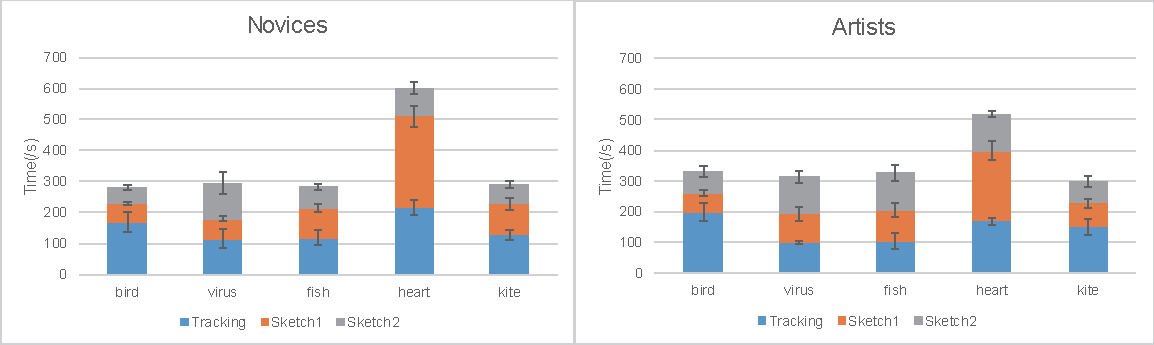
\includegraphics[width=\linewidth]{images/userstudytime3}
	\caption{Finishing time of Pilot Study I, for novice (left) and artist (right) users. Tracking: motion extraction time; Sketch1 and sketch2: motion transfer times for sketch1 and sketch2. There was no significant difference between novice and artist users.}
	\label{fig:userstudytime}
\end{figure}
\begin{figure}
	\centering
	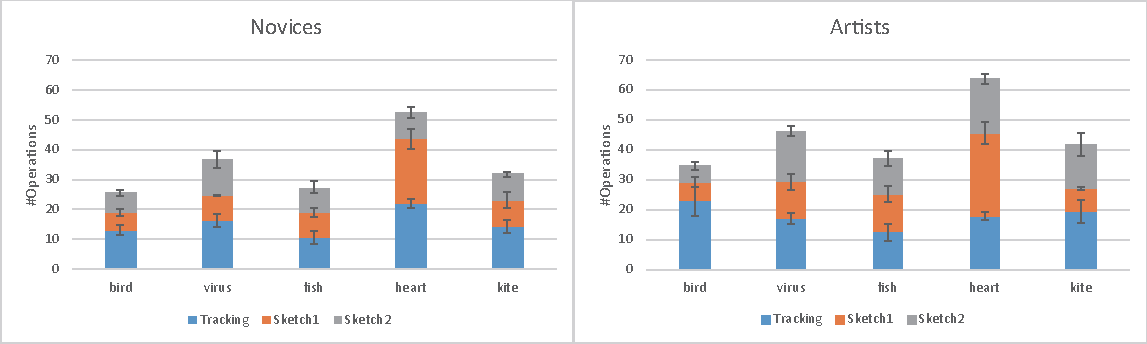
\includegraphics[width=\linewidth]{images/userstudyoperation3}
	\caption{
		The number of manual operations in Pilot Study I, for novice (left) and artist (right) users. Artists in general provided more manual operations to improve the animation quality. 	}
	\label{fig:userstudyoperation}
\end{figure}

\subsection{Pilot Study II}\label{sec:userstudy2}

In the second study, we asked the subjects who have good drawing skills (a1 to a6) from Study I to freely draw two sketches for each video used in Study I and animate them using their extracted motion in Study I. The motion could be edited or re-extracted if desired. % We then asked the user to rate the system. 
Some selected sketches drawn in this study are shown in Fig.~\ref{fig:us2sketch}, revealing a large variation both in drawing styles and in the level of details. 
The results show that our system can support users' drawing creativity reasonable well, despite using only 5 input videos.

We also collected user feedback after they finished the study, by filling out a questionnaire about their experience with both the motion extraction and motion transfer components of the system. Overall the participants were satisfied with our system. Five out of six participants mentioned the motion extraction tool was easy to learn and use. There were also five users who liked the fact that they did not need to control the animation frame-by-frame. However, four users also pointed out some limitations of the results. For example, our system might produce unexpected results when tracking points were located in smooth image regions. It also cannot produce good animation when the object of interest undergoes a 3D rotation, which is a fundamental limitation of the system as it does not know anything about 3D. 

We also asked the artists to comment on the alternative tools they might use to create such animations, and how long it would take by estimation. They mentioned a couple of commercial animation software like \emph{Adobe Flash}, \emph{Toom Boom}, but they estimated a much longer time (from one to several hours) might be needed to create similar animations with existing tools, since they would have to manually deform the input drawing or redraw it frame by frame. We are interested in conducting a more formal comparative study against these tools in the future.
 
\if 0 
\begin{figure}
	\centering
	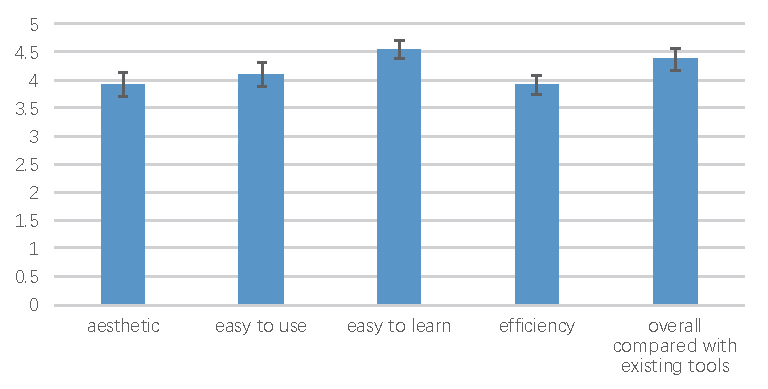
\includegraphics[width=\linewidth]{images/feedback}
	\caption{User feedback. All quantities are expressed as mean $ \pm $ standard deviation in 5 point. }
	\label{fig:feedback}
\end{figure}
\fi

\begin{figure}
	\centering
	\includegraphics[width=\linewidth]{images/us2sketch2}
	\caption{Selected sketches from Pilot Study II. Each row is a collection of one artist's work. The columns correspond to the tasks in Fig.~\ref{fig:tasks}.}
	\label{fig:us2sketch}
\end{figure}

\begin{table*}[]
	\centering
	\caption{Timings of Pilot Study I. ``tracking'', ``sketch1'', ``sketch2'' refer to the average tracking time and animation time for each input sketch in seconds, respectively.}
	\label{table:timings}
	\begin{tabular}{c|c|cccc|cccc}
		\hline
		&         & \multicolumn{4}{c}{Artist}                                  & \multicolumn{4}{|c}{Novice}                                 \\ \hline
		video & \#frame & \#control points & tracking (s) & sketch1(s) & sketch2(s) & \#control points & tracking(s) & sketch1(s) & sketch2(s) \\ \hline
		bird  & 45      & 4.7      			& 198.6547     & 62.1088     & 69.89383    & 4.2         & 169.5982     & 59.1895     & 52.06267    \\
		virus & 18      & 9.5              & 100.1268     & 92.02217    & 121.385     & 8.3         & 115.0775     & 65.71083    & 114.1543    \\
		fish  & 118     & 8                & 103.3173     & 101.2937    & 121.1722    & 6.7         & 118.7607     & 94.93717    & 69.52433    \\
		heart & 31      & 8                & 168.7968     & 229.32      & 122.1046    & 10               & 217.5835     & 291.8997    & 91.66283    \\
		kite  & 129     & 4.8      			& 150.2277     & 77.24233    & 71.84567    & 5                & 128.2655     & 99.9025     & 61.71783    \\ \hline
	\end{tabular}
\end{table*}